\section{Vehicle Routing Problem}
\label{sec:appendix_vrp}
The Capacitated Vehicle Routing Problem (CVRP) is a generalization of the TSP in which case there is a depot and multiple routes should be created, each starting and ending at the depot. In our graph based formulation, we add a special depot node with index 0 and coordinates $\mathbf{x}_0$. A vehicle (route) has capacity $D > 0$ and each (regular) node $i \in \{1, \ldots n\}$ has a demand $0 < \delta_i \le D$.  Each route starts and ends at the depot and the total demand in each route should not exceed the capacity, so $\sum_{i\in R_j} \delta_i \le D$, where $R_j$ is the set of node indices assigned to route $j$. Without loss of generality, we assume a normalized $\hat{D} = 1$ as we can use normalized demands $\hat{\delta}_i = \frac{\delta_i}{D}$.

The Split Delivery VRP (SDVRP) is a generalization of CVRP in which every node can be visited multiple times, and only a subset of the demand has to be delivered at each visit. Instances for both CVRP and SDVRP are specified in the same way: an instance with size $n$ as a depot location $\mathbf{x}_0$, $n$ node locations $\mathbf{x}_i, i = 1 \ldots n$ and (normalized) demands $0 < \hat{\delta}_i \le 1, i = 1 \ldots n$.

\subsection{Instance generation}
We follow \citet{nazari2018reinforcement} in the generation of instances for $n = 20, 50, 100$, but normalize the demands by the capacities. The depot location as well as $n$ node locations are sampled uniformly at random in the unit square. The demands are defined as $\hat{\delta}_i = \frac{\delta_i}{D^n}$ where $\delta_i$ is discrete and sampled uniformly from $\{1, \ldots, 9\}$ and $D^{20} = 30$, $D^{50} = 40$ and $D^{100}$ = 50.

\subsection{Attention Model for the VRP}

\paragraph{Encoder}
In order to allow our Attention Model to distinguish the depot node from the regular nodes, we use separate parameters $W_0^{\text{x}}$ and $\mathbf{b}_0^{\text{x}}$ to compute the initial embedding $\mathbf{h}_0^{(0)}$ of the depot node. Additionally, we provide the normalized demand $\delta_i$ as input feature (and adjust the size of parameter $W^{\text{x}}$ accordingly):
\begin{equation}
\mathbf{h}_i^{(0)} = \begin{cases}
		W_0^{\text{x}} \mathbf{x}_i + \mathbf{b}_0^{\text{x}} & i = 0 \\
        W^{\text{x}} \left[\mathbf{x}_i, \hat{\delta}_i\right] + \mathbf{b}^{\text{x}} & i = 1, \ldots, n.
\end{cases} \\
\end{equation}

\paragraph{Capacity constraints}
To facilitate the capacity constraints, we keep track of the remaining demands $\hat{\delta}_{i,t}$ for the nodes $i \in \{1, \ldots n\}$ and remaining vehicle capacity $\hat{D}_t$ at time $t$. At $t = 1$, these are initialized as $\hat{\delta}_{i,t} = \hat{\delta}_i$ and $\hat{D}_t = 1$, after which they are updated as follows (recall that $\pi_t$ is the index of the node selected at decoding step $t$):
\begin{equation}
	\hat{\delta}_{i,t+1} = \begin{cases}
		\max(0, \hat{\delta}_{i,t} - \hat{D}_t) & \pi_{t} = i \\
        \hat{\delta}_{i,t} & \pi_{t} \neq i \\
\end{cases} \\
\end{equation}
\begin{equation}
	\hat{D}_{t+1} = \begin{cases}
		\max(\hat{D}_t - \hat{\delta}_{\pi_t, t}, 0) & \pi_t \neq 0 \\
        1 & \pi_t = 0.
\end{cases} \\
\end{equation}

If we do not allow split deliveries, $\hat{\delta}_{i,t}$ will be either 0 or $\hat{\delta}_{i}$ for all $t$.

\paragraph{Decoder context}
The context for the decoder for the VRP at time $t$ is the current/last location $\pi_{t-1}$ and the remaining capacity $\hat{D}_t$. Compared to TSP, we do not need placeholders if $t=1$ as the route starts at the depot and we do not need to provide information about the first node as the route should end at the depot:
\begin{equation}
	\mathbf{h}_{(c)}^{(N)} = \begin{cases}
		\left[\bar{\mathbf{h}}^{(N)} , \mathbf{h}^{(N)}_{\pi_{t-1}} , \hat{D}_t \right] & t > 1 \\
        \left[\bar{\mathbf{h}}^{(N)} , \mathbf{h}^{(N)}_0 , \hat{D}_t \right] & t = 1.
\end{cases} \\
\end{equation}

\paragraph{Masking}
The depot can be visited multiple times, but we do not allow it to be visited at two subsequent timesteps. Therefore, in both layers of the decoder, we change the masking for the depot $j = 0$ and define $u_{(c)0} = - \infty$ if (and only if) $t = 1$ or $\pi_{t-1} = 0$. The masking for the nodes depends on whether we allow split deliveries. Without split deliveries, we do not allow nodes to be visited if their remaining demand is 0 (if the node was already visited) or exceeds the remaining capacity, so for $j \neq 0$ we define $u_{(c)j} = - \infty$ if (and only if) $\hat{\delta}_{i,t} = 0 \text{ or } \hat{\delta}_{i,t} > \hat{D}_t$. With split deliveries, we only forbid delivery when the remaining demand is 0, so we define $u_{(c)j} = - \infty$ if (and only if) $\hat{\delta}_{i,t} = 0$.

\paragraph{Split deliveries}
Without split deliveries, the remaining demand $\hat{\delta}_{i,t}$ is either 0 or $\hat{\delta}_i$, corresponding to whether the node has been visited or not, and this information is conveyed to the model via the masking of the nodes already visited. However, when split deliveries are allowed, the remaining demand $\hat{\delta}_{i,t}$ can take any value $0 \le \hat{\delta}_{i,t} \le \hat{\delta}_i$. This information cannot be included in the context node as it corresponds to individual nodes. Therefore we include it in the computation of the keys and values in both the attention layer (glimpse) and the output layer of the decoder, such that we compute queries, keys and values using:
\begin{equation}
\label{eq:dec_qkv_vrp}
	\mathbf{q}_{(c)} = W^Q \mathbf{h}_{(c)} \quad \mathbf{k}_i = W^K \mathbf{h}_i + W_d^K \hat{\delta}_{i,t}, \quad \mathbf{v}_i = W^V \mathbf{h}_i + W_d^V \hat{\delta}_{i,t}.
\end{equation}
Here we $W_d^K$ and $W_d^V$ are $(d_k \times 1)$ parameter matrices and we define $\hat{\delta}_{i,t} = 0$ for the depot $i=0$. Summing the projection of both $\mathbf{h}_i$ and $\hat{\delta}_{i,t}$ is equivalent to projecting the concatenation $[\mathbf{h}_i, \hat{\delta}_{i,t}]$ with a single $((d_h + 1) \times d_k)$ matrix $W^K$. However, using this formulation we only need to compute the first term once (instead for every $t$) and by the weight initialization this puts more importance on $\hat{\delta}_{i,t}$ initially (which is otherwise just 1 of $d_h + 1 = 129$ input values).

\paragraph{Training}
For the VRP, the length of the output of the model depends on the number of times the depot is visited. In general, the depot is visited multiple times, and in the case of SDVRP also some regular nodes are visited twice. Therefore the length of the solution is larger than $n$, which requires more memory such that we find it necessary to limit the batch size $B$ to 256 for $n = 100$ (on 2 GPUs). To keep training times tractable and the total number of parameter updates equal, we still process 2500 batches per epoch, for a total of 0.64M training instances per epoch.

\subsection{Details of baselines}
For LKH3\footnote{\url{http://akira.ruc.dk/~keld/research/LKH-3/}} by \citet{helsgaun2017extension} we build and run their code with the $\texttt{SPECIAL}$ parameter as specified in their CVRP runscript\footnote{$\texttt{run\_CVRP}$ in \url{http://akira.ruc.dk/~keld/research/LKH-3/BENCHMARKS/CVRP.tgz}}. We perform 1 run with a maximum of 10000 trials, as we found performing 10 runs only marginally improves the quality of the results while taking much more time.

\subsection{Example solutions}
\label{sec:appendix_vrp_examples}
Figure \ref{fig:cvrp_examples} shows example solutions for the CVRP with $n = 100$ that were obtained by a single construction using the model with greedy decoding. These visualizations give insight in the heuristic that the model has learned. In general we see that the model constructs the routes from the bottom to the top, starting below the depot. Most routes are densely packed, except for the last route that has to serve some remaining (close to each other) customers. In most cases, the node in the route that is farthest from the depot is somewhere in the middle of the route, such that customers are served on the way to and from the farthest nodes. In some cases, we see that the order of stops within some individual routes is suboptimal, which means that the method will likely benefit from simple further optimizations on top, such as a beam search, a post-processing procedure based on local search (e.g. 2OPT) or solving the individual routes using a TSP solver.

\begin{figure}
    \centering
    \begin{subfigure}[b]{0.49\linewidth}
        \centerline{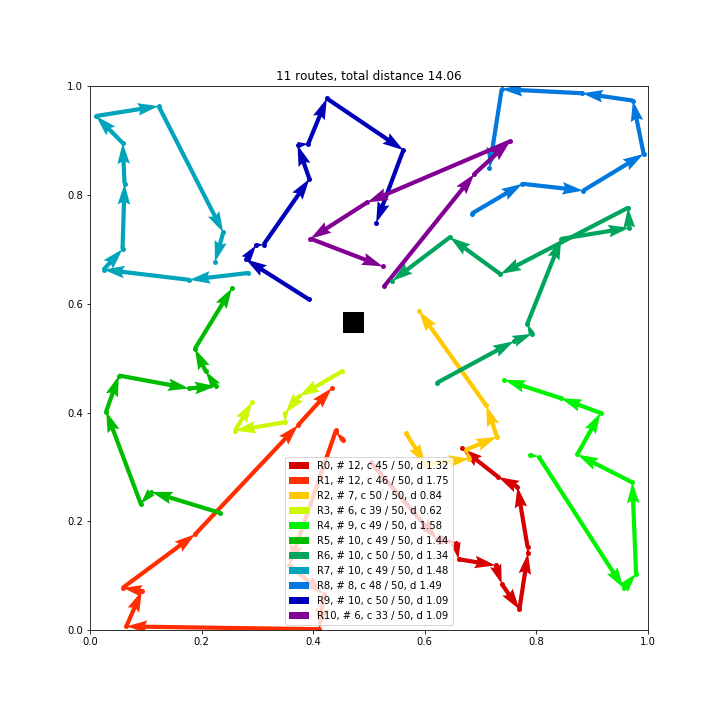
\includegraphics[trim={50 70 50 50},clip,width=\linewidth]{./images/cvrp_0}}
\caption{}
    \end{subfigure}
    ~
    \begin{subfigure}[b]{0.49\linewidth}
        \centerline{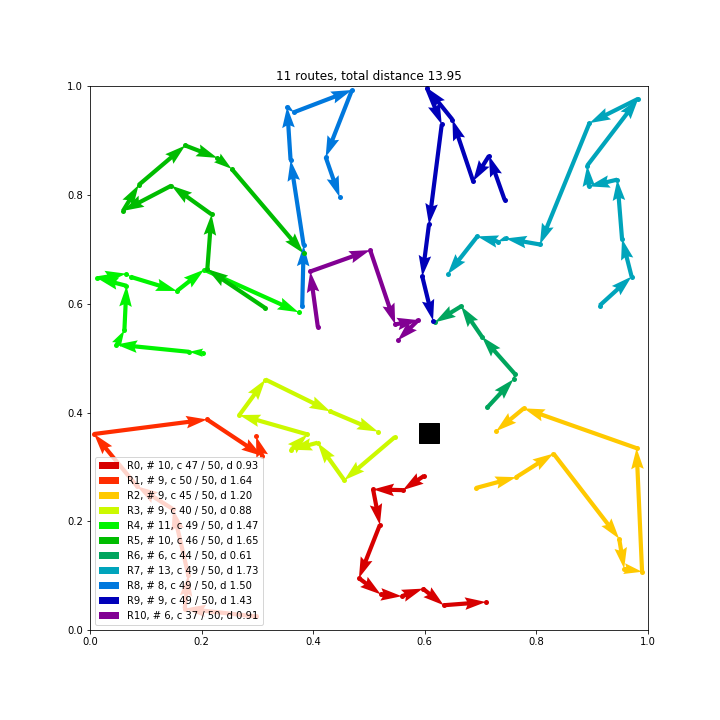
\includegraphics[trim={50 70 50 50},clip,width=\linewidth]{./images/cvrp_1}}
\caption{}
    \end{subfigure}
    
    \begin{subfigure}[b]{0.49\linewidth}
        \centerline{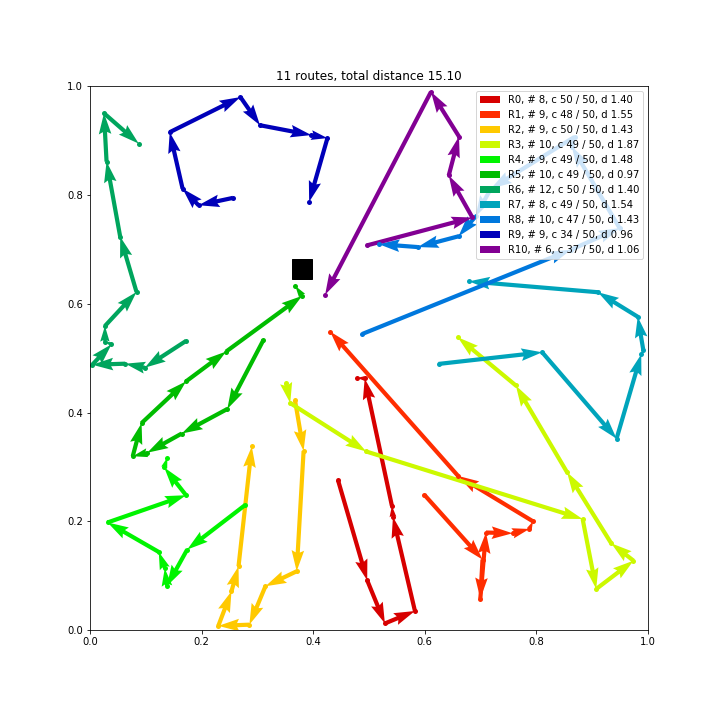
\includegraphics[trim={50 70 50 50},clip,width=\linewidth]{./images/cvrp_2}}
\caption{}
    \end{subfigure}
    ~
    \begin{subfigure}[b]{0.49\linewidth}
        \centerline{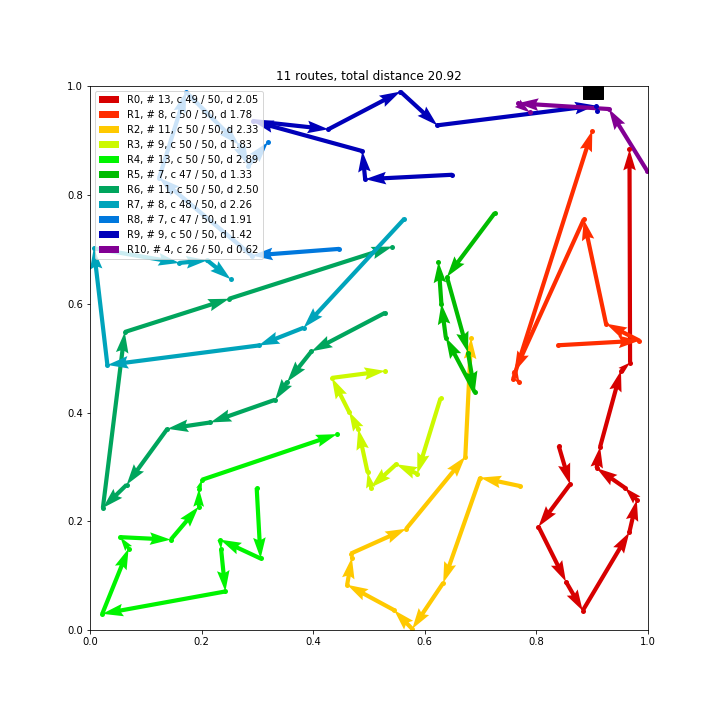
\includegraphics[trim={50 70 50 50},clip,width=\linewidth]{./images/cvrp_3}}
\caption{}
    \end{subfigure}
    
    \begin{subfigure}[b]{0.49\linewidth}
        \centerline{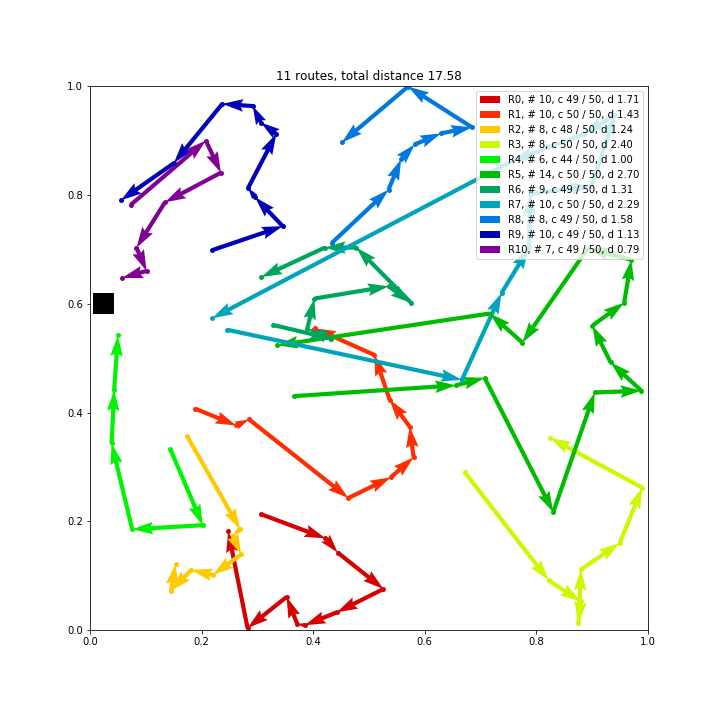
\includegraphics[trim={50 70 50 50},clip,width=\linewidth]{./images/cvrp_4}}
\caption{}
    \end{subfigure}
    ~
    \begin{subfigure}[b]{0.49\linewidth}
        \centerline{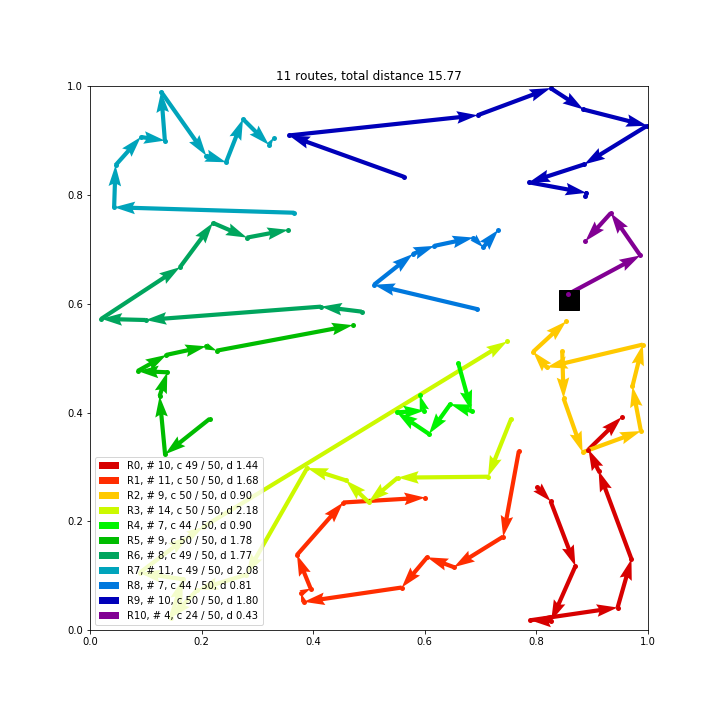
\includegraphics[trim={50 70 50 50},clip,width=\linewidth]{./images/cvrp_5}}
\caption{}
    \end{subfigure}
    \caption{Example greedy solutions for the CVRP ($n=100$). Edges from and to depot omitted for clarity. Legend order/coloring and arcs indicate the order in which the solution was generated. Legends indicate the number of stops, the used and available capacity and the distance per route.}\label{fig:cvrp_examples}
\end{figure}